\section{Control Charts}
\noindent\rule[\linienAbstand]{\linewidth}{\linienDickeDick}
The basis of a control chart is a statistical hypothesis test.

\subsection{Hypothesis test}
\noindent\rule[\linienAbstand]{\linewidth}{\linienDicke}
With a hypothesis test we want to check if an assumption (hypothesis) correct. In the case of control charts we usually want to check wheter the process is under controll. We assume that the process is under controll, meaning that the estimated mean $\bar{x}$ is equal to the target mean $\mu_0$.\\
The corresponding Hypothesis look as follows:
\begin{equation}
  \begin{split}
    H_0:& \mu_0 = \bar{x} \text{ i.e. process is not disturbed}\\
    H_1:& \mu_0 \neq \bar{x} \text{ i.e. process is disturbed}
  \end{split}
\end{equation}

To check the $H_0$ hypothesis we use a test statistic. Depending on the circumstances we use a diferent test statistic. If the standard deviation $\sigma$ is known, we use a $z$-test. If the standard deviation is unknown, a $t$-test is used.\\

\textbf{Test statistic} (z-test, since $\sigma$ is known)\\
The difference between the estimated mean and the target mean $|\bar{x} - \mu_0|$ in units of standard deviations is given by
\begin{equation}
  z = \frac{\bar{x}-\mu_0}{\sigma}\sqrt{n}.
\end{equation}

Given a confidence level (for example $\alpha = 0.0027$) we can calculate the critical difference of the estimated mean from the target mean (again in units of standard deviations), for which $H_0$ stays true with the given confidence. For $\alpha = 0.0027$ the critical distance is 3 standard deviations, $(z_q \approx 3)$. i.e. the probability of getting a more extream result (more than 3 standard deviations difference) is $0.27\%$\\

\textbf{Statistical conclusion}\\
If $|z| \leq z_q \rightarrow$ accept null hypothesis, i.e. process is not disturbed.\\
If $|z|   <  z_q \rightarrow$ reject null hypothesis, i.e. process is disturbed.\\


\textbf{Control limits}
With the critical distance $z_q$ we can calculate the control limits
\begin{equation}
  UCL = \mu_0 + z_q \frac{\sigma}{\sqrt{n}} \;\;\;\;\; LCL = \mu_0 - z_q \frac{\sigma}{\sqrt{n}}
\end{equation}

\textbf{Statistical conclusion}\\
If $LCL \leq \bar{x} \leq UCL \rightarrow$ process is not disturbed.\\
If $\bar{x} < LCL \;\text{or}\; UCL < \bar{x} \rightarrow$ process is disturbed.\\

\subsection{The Control Chart}
\noindent\rule[\linienAbstand]{\linewidth}{\linienDicke}
We introduce the most commonly used Shewhart control chart for monitoring the mean and the variation of a process. First and foremost, we are interested in monitoring the variation, and only in the second instance, if the variation is under control, we will consider the chart for the mean.
\begin{figure}[H]
  \centering
  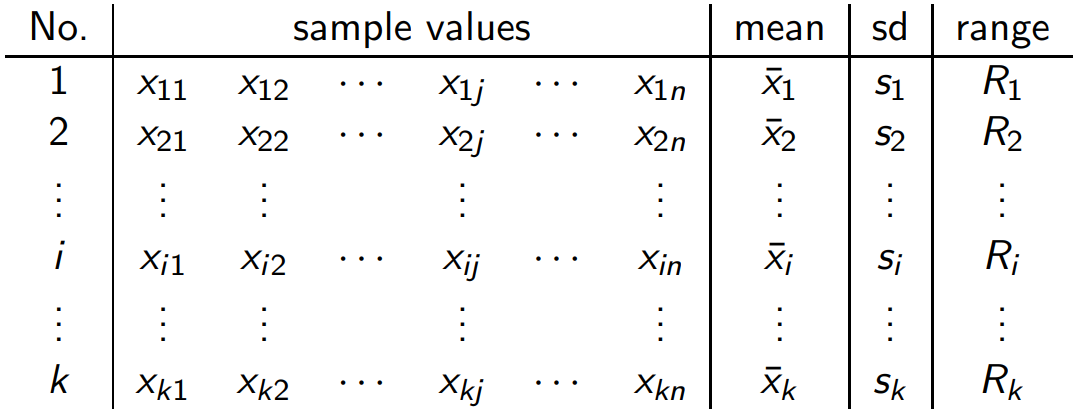
\includegraphics[width = 0.8\linewidth]{Pics/2.1.png}
  \caption{Data Set with Mean, Standard Deviation and Range}
  \label{2.1}
\end{figure}

\textbf{Mean values}
\begin{equation}
  \bar{x}_i = \frac{1}{n} \sum_{j=1}^n x_{ij}
\end{equation}

\textbf{Standard deviations}
\begin{equation}
  s_i = \sqrt{\frac{1}{n-1} \sum_{j=1}^n \left(x_{ij} - \bar{x}_i\right)^2}
\end{equation}

\textbf{Ranges}
\begin{equation}
  R_i = max\left \{x_{ij} | j \in \left \{1,...,n\right \} \right \} - min\left \{x_{ij} | j \in \left \{1,...,n\right \} \right \}
\end{equation}

% \subsection{R Chart}
% \noindent\rule[\linienAbstand]{\linewidth}{\linienDicke}
\subsection{Control Charts for $\bar{x}$ and R}
\noindent\rule[\linienAbstand]{\linewidth}{\linienDicke}
Firs we monitor the variation of the process with the R- Chart. If the variation is under control, we will consider the chart for
the mean $\bar{x}$.\\
\paragraph{R-Chart}\mbox{}\\
\textbf{Centerline}\\
The centreline (CL) of the $R$ chart is denoted by $\bar{R}$ and is calculated from the arithmetic mean of the ranges of the $k$ random samples, i.e.
\begin{equation}
  \bar{R} = \frac{1}{k} \sum^k_{i=1} R_i
\end{equation}

\textbf{Control limits}\\
\begin{equation}
    UCL = D_4 \bar{R}; \;\;\;\;\; LCL = D_3 \bar{R}
\end{equation}
The constants $D_3$ and $D_4$ depend only on the sample size $n$ and can be found in tables.

\paragraph{$\bar{x}$ Chart based on R chart}\mbox{}\\
% \subsection{$\bar{x}$ Chart based on R chart}
% \noindent\rule[\linienAbstand]{\linewidth}{\linienDicke}
\textbf{Control limits}\\
The control limits of the $\bar{x}$ chart can be calculated using the mean $\mu$, the standard error and the significance level of $z_q = 3$.
\begin{equation}
  \begin{split}
    UCL = \mu + 3 \frac{\sigma}{\sqrt{n}}; \;\;\;\;\; LCL = \mu - 3 \frac{\sigma}{\sqrt{n}}
  \end{split}
\end{equation}
The problem with that is that $\mu$ and $\sigma$ are in general unknown and must be estimated from the process data.\\
This is a two-stage process. First make sure that the process standard deviation (R chart) is under statistical control. That is, if some samples are out of bounds, it is recommended to omit these measurements and recalculate the limits. Next we can use $\bar{R}$ to estimate the process standard deviation.\\
\begin{equation}
  \hat{\sigma} = \frac{\bar{R}}{d_2}
\end{equation}

% \textbf{Centerline}\\
% We know that for an independent sample $x_1, ... ,x_n$ from a normal distribution with parameters $\mu$ and $\sigma$ the mean
% \begin{equation}
%   \bar{x} = \frac{1}{n} \sum_{j=1}^n x_{j}
% \end{equation}
% satisfies
% \begin{equation}
%   E\left(\bar{x}\right) = \mu \;\;\;\; and \;\;\;\; Var\left(\bar{x}\right) = \frac{\sigma^2}{n}
% \end{equation}
%
% The mean is an unbiased estimator with the standard error
% \begin{equation}
%   SE\left(\bar{x}\right) = \frac{\sigma}{\sqrt{n}}
% \end{equation}
%
% Assumption: R chart is under statistical control.\\
%  - The value $\bar{R}$ is a reliable estimate for the mean range.\\
%  - The value $\bar{R}$ is a reliable estimate for the process standard deviation
% \begin{equation}
%   \hat{\sigma} = \frac{\bar{R}}{d_2}
% \end{equation}

\textbf{Centerline}\\
Any samples excluded for construction of the R chart should also be disregarded for construction of the $\bar{x}$ chart.
This results in a sample of $k^\star$ valid samples, (where $k^\star$ denotes the reduced number of samples).
Mean values of $\bar{x}_1, ... ,\bar{x}_{k^\star}$ provide an estimate of $\mu$, i.e
\begin{equation}
  \bar{\bar{x}} = \frac{1}{k^\star} \sum^{k^\star}_{i=1} \bar{x_i}
\end{equation}

\textbf{Control limits}\\
The control limits then are
\begin{equation}
  \begin{split}
    UCL =& \bar{\bar{x}} + 3\frac{\bar{R}}{d_2} \frac{1}{\sqrt{n}}\approx \bar{\bar{x}} + A_2 \bar{R}\\
    UCL =& \bar{\bar{x}} - 3\frac{\bar{R}}{d_2} \frac{1}{\sqrt{n}}\approx \bar{\bar{x}} - A_2 \bar{R}
  \end{split}
\end{equation}

\subsection{Control Chart with $\bar{x}$ and s}
\noindent\rule[\linienAbstand]{\linewidth}{\linienDicke}
We again monitor the variation (this time with an s chart) and then consider the chart for the mean $\bar{x}$.
\paragraph{s Chart}\mbox{}\\
\textbf{Centerline}\\
The centreline of the s chart is denoted by $\bar{s}$ and is calculated from the arithmetic mean of the standard deviations\\
\begin{equation}
  \bar{s} = \frac{1}{k} \sum^k_{i=1} s_i
\end{equation}

\textbf{Control limits}\\
Analogously to above, the control limits are given by
\begin{equation}
    UCL = B_4 \bar{s}; \;\;\;\;\; LCL = B_3 \bar{s}
\end{equation}

\paragraph{$\bar{x}$ Chart based on s chart}\mbox{}\\
Using an s chart of a process that is under control, the process standard deviation can be estimated by
\begin{equation}
  \hat{\sigma} = \frac{\bar{s}}{c_4}
\end{equation}
\textbf{Centerline}\\
Any samples excluded for construction of the s chart should again also be disregarded for construction of the $\bar{x}$ chart.
This results in a sample of $k^\star$ valid samples, (where $k^\star$ denotes the reduced number of samples).
Mean values of $\bar{x}_1, ... ,\bar{x}_{k^\star}$ provide an estimate of $\mu$, i.e
\begin{equation}
  \hat{\mu} = \bar{\bar{x}} = \frac{1}{k^\star} \sum^{k^\star}_{i=1} \bar{x_i}
\end{equation}

\textbf{Control limits}
\begin{equation}
  \begin{split}
    UCL =& \bar{\bar{x}} + 3\frac{\bar{s}}{c_4} \frac{1}{\sqrt{n}} \approx \bar{\bar{x}} + A_3 \bar{s}\\
    UCL =& \bar{\bar{x}} - 3\frac{\bar{s}}{c_4} \frac{1}{\sqrt{n}} \approx \bar{\bar{x}} - A_3 \bar{s}
  \end{split}
\end{equation}

\subsection{Individual Control Charts}
\noindent\rule[\linienAbstand]{\linewidth}{\linienDicke}
Individual control charts have exactly one measurement per sample.\\
The problem with that is that one cannot estimate variability from a single measurement. The solution to that is to use variation of two adjacent measurements to measure the process variability.\\

The moving range is defined as
\begin{equation}
  MR_i = |x_{i+1} - x_i|
\end{equation}
for all $i \in \left\{1,...,n-1\right\}$.\\

The arithmetic mean of all moving ranges
\begin{equation}
  \overline{MR} = \frac{1}{n-1} \sum_{i=1}^{n-1}MR_i
\end{equation}
is a reasonable estimate for the process standard deviation
\begin{equation}
  \hat{\sigma} = \frac{\overline{MR}}{d_2} = \frac{\overline{MR}}{1.128}
\end{equation}
Since two neighboring measurements were used to calculate the moving ranges we have $d_2 = 1.128$.\\

\textbf{Centerline}\\
The centerline for the individuals control chart is the arithmetic mean of the measured values.
\begin{equation}
  \bar{x} = \frac{1}{k} \sum^k_{i=1} x_i
\end{equation}

\textbf{Control limits}
\begin{equation}
    UCL = \bar{x} + 3 \frac{\overline{MR}}{1.128}; \;\;\;\;\; LCL = \overline{x} - 3 \frac{\overline{MR}}{1.128}
\end{equation}

\subsection{Control Charts for Attributes Data – p Chart}
\noindent\rule[\linienAbstand]{\linewidth}{\linienDicke}
Sometimes it is useful to mark a product as defective or useable. In such a case we need a control chart for attributes data.\\

We consider a sample of size $n$ and find $D$ broken parts. The number of defective $D$ under $n$ examined parts is known to be binomial distributed with the unknown probability of success. The relative frequency
\begin{equation}
  \hat{p} = \frac{D}{n}
\end{equation}
is an estimator of the unknown probability of success $p$. In addition, the variance of the estimator $\hat{p}$ is given by
\begin{equation}
  Var(\hat{p}) = \frac{p(1-p)}{n}
\end{equation}
Given $k$ samples with $n_1,...,n_k$ values. Each of these samples has $d_1,...,d_k$ defective products. That is, we get $k$ relative frequencies
\begin{equation}
  p_1 = \frac{d_1}{n_1},...\;,p_k = \frac{d_k}{n_k}
\end{equation}
which we plot against the index i in a scatter plot.\\

The centreline and the control limits of a p chart are again determined from a stable trial run with $k^\star$ valid samples.\\
\begin{itemize}
  \item If the sample sizes $n_1,...,n_k$ are all equal to $n$, then the centreline is the arithmetic mean of the relative frequencies of the (reduced) trial run
  \begin{equation}
    \bar{p} = \frac{1}{k^\star} \sum^{k^\star}_{i=1}p_i
  \end{equation}
  In this case the control limits for a p chart are given by
  \begin{equation}
    UCL = \bar{p} + 3\sqrt{\frac{\bar{p}(1-\bar{p})}{n}}; \;\;\;\;\; LSL = \bar{p} - 3\sqrt{\frac{\bar{p}(1-\bar{p})}{n}}
  \end{equation}
  \item On the other hand, if the sample sizes are not all the same, the control limits also depend on the index $i$, i.e. on the respective sample size $n_i$. The centreline is then given by
  \begin{equation}
    \bar{p} = \frac{d_1 + \cdots + d_{k^\star}}{n_1 + \cdots + n_{k^\star}}
  \end{equation}
  and the control limits by
  \begin{equation}
    UCL_i = \bar{p} + 3\sqrt{\frac{\bar{p}(1-\bar{p})}{n_i}}; \;\;\;\;\; LSL_i = \bar{p} - 3\sqrt{\frac{\bar{p}(1-\bar{p})}{n_i}}
  \end{equation}
\end{itemize}
